\let\negmedspace\undefined
\let\negthickspace\undefined
\documentclass[journal]{IEEEtran}
\usepackage[a4paper, margin=10mm, onecolumn]{geometry}
\usepackage{lmodern} % Ensure lmodern is loaded for pdflatex
\usepackage{tfrupee} % Include tfrupee package

\setlength{\headheight}{1cm} % Set the height of the header box
\setlength{\headsep}{0mm}  % Set the distance between the header box and the top of the text

\usepackage{gvv-book}
\usepackage{gvv}
\usepackage{cite}
\usepackage{amsmath,amssymb,amsfonts,amsthm}
\usepackage{algorithmic}
\usepackage{graphicx}
\usepackage{float}
\usepackage{textcomp}
\usepackage{xcolor}
\usepackage{txfonts}
\usepackage{listings}
\usepackage{enumitem}
\usepackage{mathtools}
\usepackage{gensymb}
\usepackage{comment}
\usepackage[breaklinks=true]{hyperref}
\usepackage{tkz-euclide} 
\usepackage{listings}
% \usepackage{gvv}                                        
\def\inputGnumericTable{}                                 
\usepackage[latin1]{inputenc}                                
\usepackage{color}                                            
\usepackage{array}                                            
\usepackage{longtable}                                       
\usepackage{calc}                                             
\usepackage{multirow}                                         
\usepackage{hhline}                                           
\usepackage{ifthen}                                           
\usepackage{lscape}
\usepackage{tikz}
\usetikzlibrary{patterns}

\begin{document}

\bibliographystyle{IEEEtran}
\vspace{3cm}

\title{2.5.32}
\author{EE25BTECH11064 - Yojit Manral}

\maketitle
% \maketitle
% \newpage
% \bigskip
{\let\newpage\relax\maketitle}
\renewcommand{\thefigure}{\theenumi}
\renewcommand{\thetable}{\theenumi}
\setlength{\intextsep}{10pt} % Space between text and float

\textbf{Question:}\\
Show that the points $\brak{7,10}$, $\brak{-2,5}$ and $\brak{3,4}$ are vertices of an isosceles right triangle.

\textbf{Solution:}\\
\begin{table}[h!]    
  \centering
  \begin{tabular}[12pt]{ |c| c|}
    \hline
    \textbf{Points} & \textbf{Name}\\ 
    \hline
	\myvec{7\\10} & Point $\Vec{A}$ \\
    \hline 
	\myvec{-2\\5} & Point $\Vec{B}$\\
    \hline
	\myvec{3\\4} & Point $\Vec{C}$\\
    \hline
\end{tabular}
  \caption{List of Points}
  \label{Table_1}
\end{table} \\
$\rightarrow$ The equation of the sides are given as
\begin{align}
    \vec{B}-\vec{A}=\myvec{-9\\-5} && \vec{C}-\vec{B}=\myvec{5\\-1} && \vec{A}-\vec{C}=\myvec{4\\6}
\end{align}
$\rightarrow$ The medians $\vec{D}$, $\vec{E}$ and $\vec{F}$ of the triangle are
\begin{align}
    \vec{D} = \frac{\vec{A}+\vec{B}}{2} = \myvec{5/2\\15/2} &&
    \vec{E} = \frac{\vec{B}+\vec{C}}{2} = \myvec{1/2\\9/2} &&
    \vec{F} = \frac{\vec{C}+\vec{A}}{2} = \myvec{5\\7}
\end{align}
\begin{enumerate}[label=(\alph*)]
\item {
For an isosceles triangle, median to the base is also the perpendicular bisector. Using this property
\begin{align}
    (\vec{C}-\vec{D})^T(\vec{B}-\vec{A}) &= \myvec{1/2&-7/2}\myvec{-9\\-5} = 13 \neq 0 \\
    (\vec{A}-\vec{E})^T(\vec{C}-\vec{B}) &= \myvec{13/2&11/2}\myvec{5\\-1} = 27 \neq 0 \\
    (\vec{B}-\vec{F})^T(\vec{A}-\vec{C}) &= \myvec{-7&-2}\myvec{4\\6} = -40 \neq 0
\end{align}
$\rightarrow$ Since none of the sides satisfy this property, the triangle is not isosceles.
}
\item {
For a right triangle, dot product of the perpendicular sides must be zero.
\begin{align}
    (\vec{B}-\vec{A})^T(\vec{C}-\vec{B})&=\myvec{-9&-5}\myvec{5\\-1} = -40 \neq 0 \\
    (\vec{C}-\vec{B})^T(\vec{A}-\vec{C})&=\myvec{5&-1}\myvec{4\\6} = 14 \neq 0 \\
    (\vec{A}-\vec{C})^T(\vec{B}-\vec{A})&=\myvec{4&6}\myvec{-9\\-5} = -66 \neq 0
\end{align}
$\rightarrow$ Since none of the dot products is zero, no two sides are perpendicular, and the triangle is not right angled.
}
\end{enumerate}
$\longrightarrow$ From proofs (a) and (b) above, we can conclude that $\triangle ABC$ is not an isosceles right triangle.
\begin{figure}[h!]
   \centering
   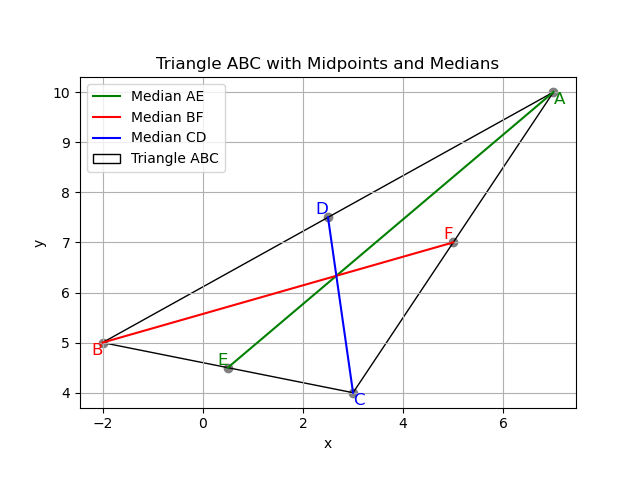
\includegraphics[width=\linewidth]{figs/01.png}
   \caption{Plot of $\triangle$ABC}
   \label{Plot_1}
\end{figure}
\end{document}
